\section{Model Simulation and Evaluation}
\label{sec:Model-Simulation-Evaluation}
\index{PerfModel!Model Simulation Evaluation}

\begin{figure}[t]
  \centering
  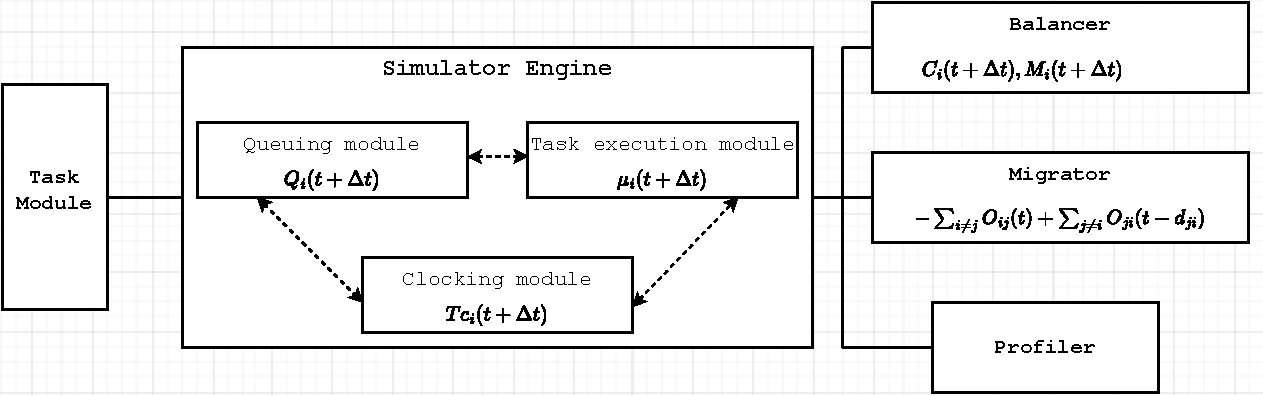
\includegraphics[scale=0.625]{./pictures/perf_analysis_model/perf_modularized_components_for_simulation_design.pdf}
	\caption{Modularized components for a simulator design following the performance model of reactive load balancing.}
	\label{fig:react_lb_sim_design}
\end{figure}

From the proposed model, this section introduces how we map its parameters to design a simulator. Figure \ref{fig:react_lb_sim_design} shows five modules corresponding to five components from left to right, including \texttt{Task Module}, \texttt{Simulator Engine}, \texttt{Balancer}, \texttt{Migrator}, and \texttt{Profiler}. The role of each module is addressed as follows.

\begin{itemize}
	\item \texttt{Task Module}: to define a task with its properties, e.g., ID, load value (or wallclock execution time, $w$), data size ($s$), local process, remote process (if a task is migrated), start time, end time, and migration time (if yes).
	
	\item \texttt{Simulator Engine}: the core of the simulator. There are three modules inside the engine, including \texttt{Queuing module}, \texttt{Task execution module}, and \texttt{Clocking module}. Clocking starts after the engine is triggered to run. It will end counting after all tasks are finished. Queuing controls task distribution and task dequeuing. In detail, each process has two types of queues, a local queue for executing local tasks and a remote queue for executing remote tasks. Task execution module manages the execution of tasks with timing, i.e., start time, execution time, and end time of a task.
	
	\item \texttt{Balancer}: the module for triggering load balancing operations. We emulate dynamic load balancing by revoking this module at every time step to make sure the condition of imbalance is checked. Therefore, if the ratio between clocking and runtime units is infinitesimal, \texttt{Balancer} can show an execution more realistic.
	
	\item \texttt{Migrator}: decides task migration based on the results of \texttt{Balancer}. This module takes care of migration time, delay, and arrival time of tasks as well as when they are executed on remote side.
	
	\item \texttt{Profiler}: performs statistics and visualization for profiling an execution by simulator.
\end{itemize}

Associated with the modularized design in Figure \ref{fig:react_lb_sim_design}, we present how the workflow of the simulator runs. The actions of all modules are linked together and controlled through each time clock (or time step). First, the simulator inputs include:
\begin{itemize}
	\item The number of tasks in total ($T$).
	\item The number of processes ($P$) with a given distribution of $T$ on $P$ processes, indicating the number of tasks on each process ($T_{i}$).
	\item The slowdown information, for example, the number of slowed down processes and how is the slowdown factor compared to the normal case ($Slow_{i}$). This value indicates execution speed ($S_{P_{i}}$) per process. Assume we have a baseline is $1.0$ tasks/time unit. Plus slowdown, it could be slowed down as $0.5$ or $0.25$ tasks/time unit.
	\item Overhead information, in balancing operation and task migration, indicate latency ($\lambda$) and bandwidth ($B$) to calculate delay time. For generalization, we denote the overhead information by two types, balancing overhead ($O_{balancing}$) and task migration overhead ($d$). $O_{balancing}$ consists of monitoring and exchanging information, $m_{i}(t, t+\Delta t)$ and $b_{i}(t - \lambda)$ respectively. $d$ represents delay time when tasks are migrated. With the data size of each task, $d$ regulates the arrival time of a migrated task.
\end{itemize}

\begin{figure}[t]
  \centering
  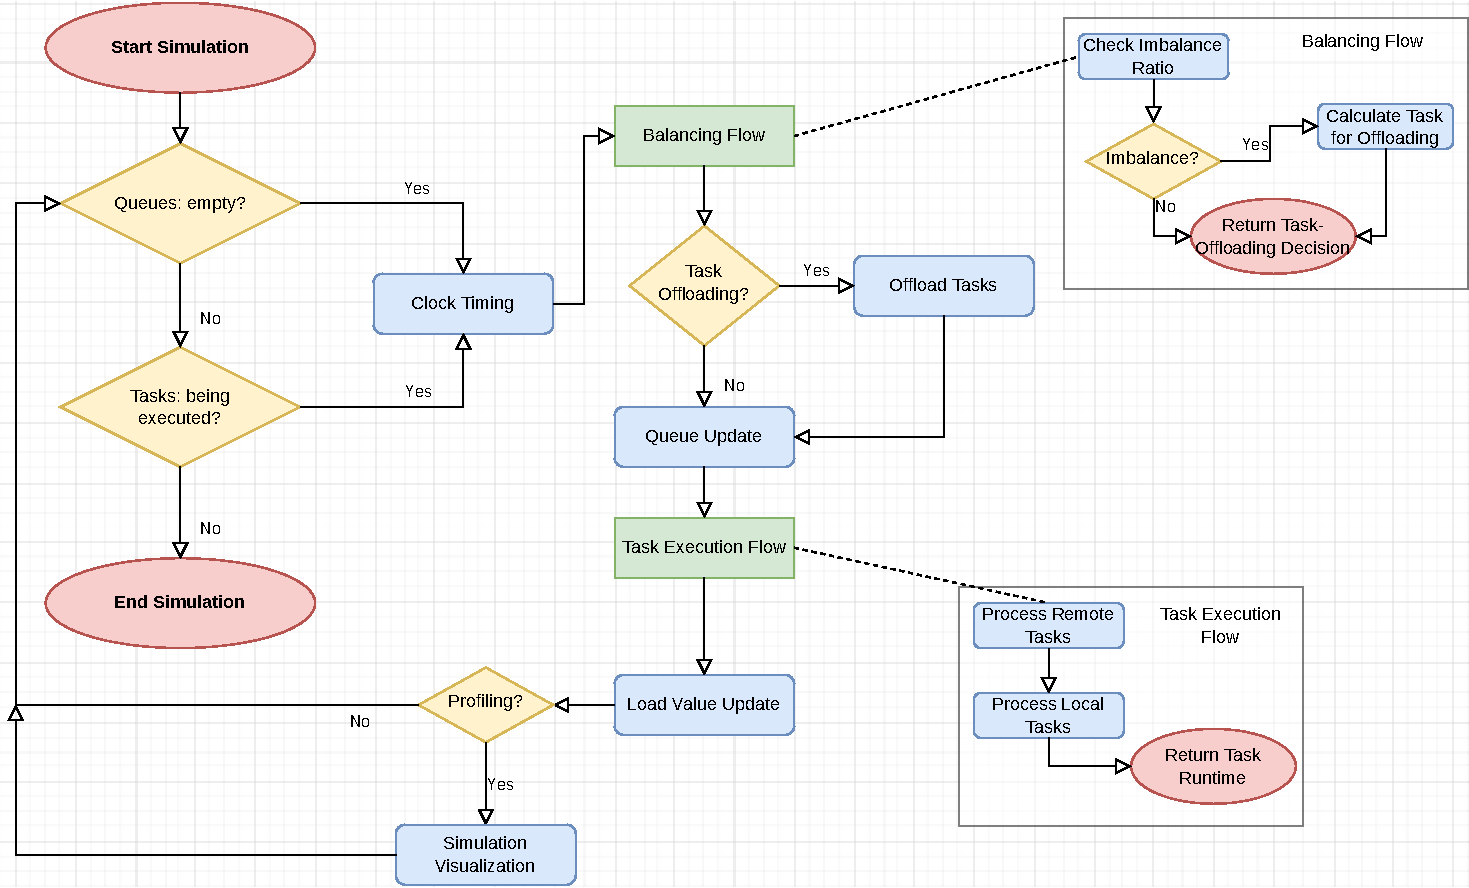
\includegraphics[scale=0.55]{./pictures/perf_analysis_model/perf_simulation_flow.pdf}
	\caption{Workflow of the simulation.}
	\label{fig:react_lb_simulator_flow}
\end{figure}

Figure \ref{fig:react_lb_simulator_flow} addresses the workflow of the simulator. The starting point opens a while loop (shown as \texttt{Start Simulatior}) with the conditions: queue length is not empty, or some tasks are being executed. If yes, the clock is ticked to simulate our scenario. ``Tick'' or ``ticking'' indicates counting time steps in the simulator. Next, we load \texttt{Balancer} denoted by a sub-flow (\texttt{Balancing Flow}). In detail, we check imbalance ratio and calculate whether tasks are offloaded or not. After that, we update all the queues if some tasks are offloaded or even if nothing is changed. The simulation engine will then load the task execution flow (\texttt{Task Execution Flow}). We prioritize remote tasks being executed first and local tasks afterward. This intends to make the simulation with the same reactive load balancing strategy from the original work proposed by Klinkenberg et al. \cite{Klinkenberg2020ChameleonReactLB}. After \texttt{Task Execution Flow}, all task properties, e.g., end-time, runtime, are updated. Typically, these properties are forwarded to \texttt{Load Value Update} to keep tracking the total load values of each process. In general, the loop repeats and ends if there are no more tasks for execution. The following subsection will explain the implementation of our simulation design as a reference simulator.

\subsection{Simulator Implementation}
\label{subsec:Simulator-Implementation}

\begin{figure}[t]
  \centering
  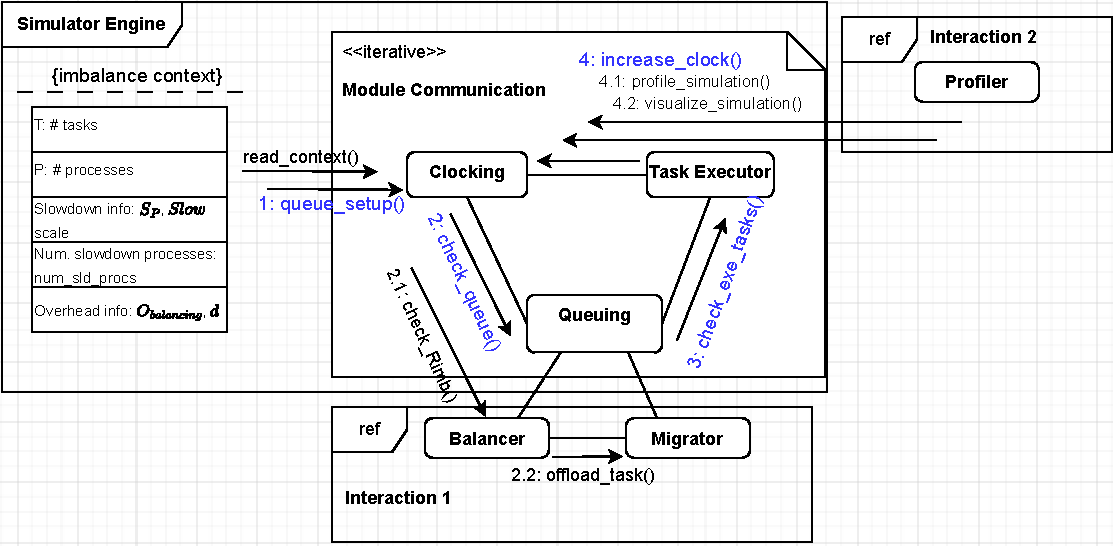
\includegraphics[scale=0.7]{./pictures/perf_analysis_model/perf_simulator_comm_diagram.pdf}
	\caption{A communication diagram of dynamic load balancing simulation.}
	\label{fig:simulator_comm_diagram}
\end{figure}

\begin{figure}[t]
  \centering
  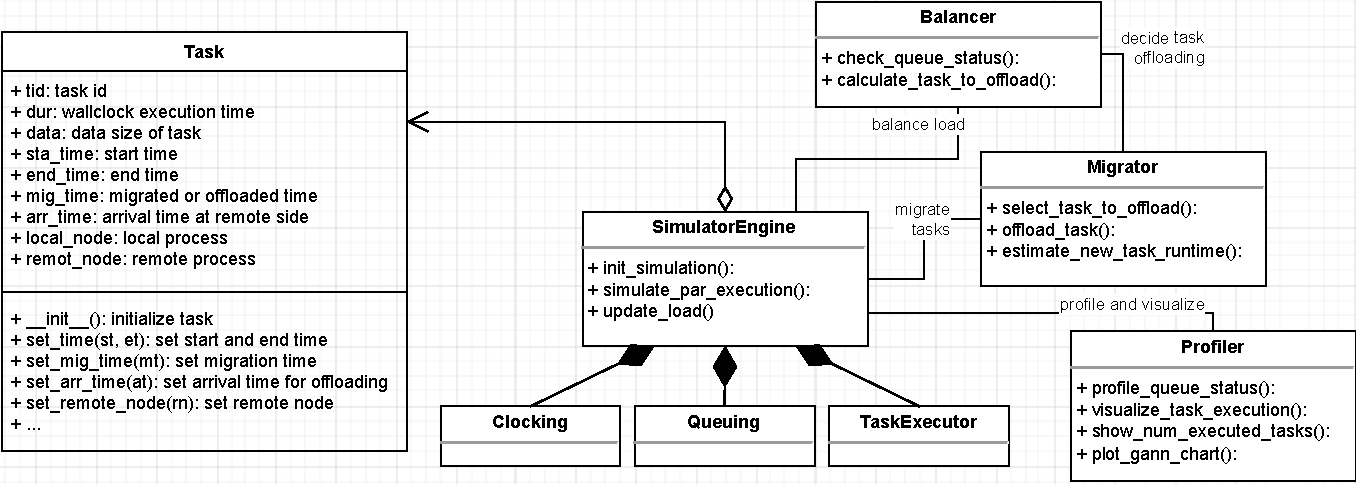
\includegraphics[scale=0.65]{./pictures/perf_analysis_model/perf_simulator_class_diagram.pdf}
	\caption{A class diagram of dynamic load balancing simulator.}
	\label{fig:simulator_class_diagram}
\end{figure}

A communication diagram and a class diagram are used to present the simulator implementation. The communication diagram shown in Figure \ref{fig:react_lb_sim_design} explains how the simulator modules communicate with each other, while the class diagram shows at a more detailed level how classes and objects are defined in the implementation. Intuitively, we show the communication and class diagrams in Figure \ref{fig:simulator_comm_diagram} and Figure \ref{fig:simulator_class_diagram}, respectively.

% --------------------------------------------
\newpage
% --------------------------------------------

The communication diagram is depicted with three main blocks: \texttt{Simulator Engine}, \texttt{Interaction 1}, and \texttt{Interaction 2}. Block \texttt{Simulator Engine} highlights the simulator input standing for the constraints of imbalance context (\texttt{{imbalance context}}). Then, it is followed by the sub-block - \texttt{Module Communication}, including \textbf{Clocking}, \textbf{Queuing}, and \textbf{Task Executor} that indicate the corresponding modules explained in Figure \ref{fig:react_lb_sim_design}. At the bottom, block \texttt{Interaction 1} contains the modules, \textbf{Balancer} and \textbf{Migrator}. On the right corner, Block \texttt{Interaction 2} contains the module, \textbf{Profiler}.\\

Initially, the input is declared by the parameters, such as $T$, $P$, slowdown information, and overhead information that are mentioned in the previous sub-section. From here, the communication of all modules in block \texttt{Simulator Engine} with the other modules in block \texttt{Interaction 1} and \texttt{Interaction 2} can be described by four main actions:
\begin{enumerate}
	\item \texttt{queue\_setup()}
	\item \texttt{check\_queue()}
	\item \texttt{check\_exe\_tasks()}
	\item \texttt{increase\_clock()}
\end{enumerate}

These actions are highlighted in blue in Figure \ref{fig:simulator_comm_diagram}, and their order is also considered as the simulation workflow.\\

\texttt{queue\_setup()} distributes tasks over the local queue of each process. Tasks are then queued and executed locally or remotely, managed by module \textbf{Queuing}. Users can adjust the setup of each queue to simulate a specific imbalance scenario.\\
	
\texttt{check\_queue()} follows by each time step from module \textbf{Clocking}, where \textbf{Clocking} accounts for ticking or counting time steps. With time units in \textbf{Clocking}, their value can be configured by a ratio between the number of time steps and the amount of time that a task is executed (task execution time). Thereby, when task migration and balancing operation overhead are set by several time units, the configured ratio can reflect the proportion of overhead over task execution time. For example, suppose task execution time is in seconds and time steps are counted in milliseconds; the ratio will be $1:1000$. If the overhead of task migration is assumed to be a few milliseconds, then the simulation engine can emulate this more realistically. There are two sub-actions inside \texttt{check\_queue()}, including \texttt{check\_Rimb()} and \texttt{offload\_task()}. If an imbalance condition is satisfied, tasks are offloaded depending on our offloading strategies. The action of task offloading is modularized as an interaction region (\texttt{Interaction 1}) where we can modify balancing algorithms and task offloading strategies.\\
	
\texttt{check\_exe\_tasks()} is a connection between \textbf{Queuing} and \textbf{Task Executor}. \textbf{Task Executor} takes tasks from the queues and simulates the execution of tasks in parallel. At a time step, all queues are checked. Tasks are executed slowly or quickly depending on the values of $S_{P_{i}}$ and $Slow_{i}$ factors that we set up, where $i$ indicates process $P_{i}$.\\
	
\texttt{increase\_clock()} simply checks and increases the time step value. The interaction region \\ (\texttt{Interaction 2}) is shown here to indicate module \textbf{Profiler}. \textbf{Profiler} supports profiling and visualizing task-by-task execution.\\

Building upon the communication diagram, we define several classes in response to the abovementioned modules. Figure \ref{fig:simulator_class_diagram} shows the class diagram, where each class is illustrated with some corresponding properties and methods. In detail, we can see classes and interfaces revealed as a reference implementation, namely \textbf{Task}, \textbf{SimulatorEngine}, \textbf{Clocking}, \textbf{Queuing}, \textbf{TaskExecutor}, \textbf{Balancer}, \textbf{Migrator}, and \textbf{Profiler}.\\

Class \textbf{Task} needs relevant properties to manage a task, such as a unique id (\texttt{tid}), wallclock execution time (\texttt{dur}), and other attributes related to time, i.e., start time (\texttt{sta\_time}), end time (\texttt{end\_time}), migrated/offloaded time (\texttt{mig\_time}). Behind the properties, there are relevant methods to setting or getting the corresponding values, e.g., \texttt{set\_time(st, et)} to set start and end time of a task, \texttt{set\_mig\_time(mt)} to set migrated time if a task is selected for offloading.\\

The main interface is \texttt{SimulatorEngine}, which has an aggregation link to class \texttt{Task}. Inside \texttt{SimulatorEngine}, we have three methods, including \texttt{init\_simulation()}, \texttt{simulate\_par\_execution()}, and \texttt{update\_load()}. \texttt{SimulatorEngine} exists a composition link with the other interfaces, \texttt{Clocking}, \texttt{Queuing}, and \texttt{TaskExecutor}. Besides that, the other association links in \texttt{SimulatorEngine} are connecting to the classes, \texttt{Balancer}, \texttt{Migrator}, and \texttt{Profiler}.\\

\texttt{Balancer} aims to check all the queue's status over time steps (by the method \texttt{check\_queue\_status()}), which is used to calculate imbalance ratio. If $R_{imb}$ is satisfied a given threshold (condition), then \texttt{calculate\_task\_to\_offload()} is invoked to decide offloading tasks.\\

Associated with \texttt{Migrator}, our implementation goes into the methods of \texttt{select\_task\_to\_offload()}, \texttt{offload\_task()}, \texttt{estimate\_new\_task\_runtime()} to perform task offloading. Within this class, the properties, called \texttt{mig\_time} and \texttt{arr\_time}, are updated to fit the specification about balancing operation overhead and task migration overhead. Optionally, class \texttt{Profiler} is defined to support profiling and visualizing the execution behavior of the simulator.

\subsection{Example Simulator Run}
\label{subsec:Simulator-Run-Example}

This sub-section provides an illustrative example of running the simulator. We re-use the the imbalance scenario in Figure \ref{fig:k_estimation_avg_bound} (B) on Page \pageref{fig:k_estimation_avg_bound}, Scenario $1$. In particular, the simulation example is configured by applying reactive load balancing. Scenario $1$ is set up $8$ processes, $R_{imb} = 1.5$. There are two processes slowed down by the scale of $5 \times$. Assuming the simulation configuration for baseline processes is an execution rate of $1.0\ \text{tasks/time unit}$, while the two slow processes execute tasks with a rate of $0.2\ \text{tasks/time unit}$. We configure time units in milliseconds and task execution in seconds. The ratio between task execution time and balancing time step is $1:1000$. To provide a more realistic simulation, we make some assumptions about the runtime of local tasks and remote tasks as follows.
\begin{itemize}
	\item For a remote task offloaded from a slow process to a fast one, its execution time is considered a half decrease compared to running on the original process. The reason is the constraint of performance slowdown on the original process.
	\item For a remote task offloaded from a fast process to a slow one, its execution time on the side of slow processes is slow as the local tasks.
	\item For a remote task offloaded from fast-to-fast or slow-to-slow, its execution time is assumed not to be changed.
\end{itemize}

\begin{figure}[t]
  \centering
  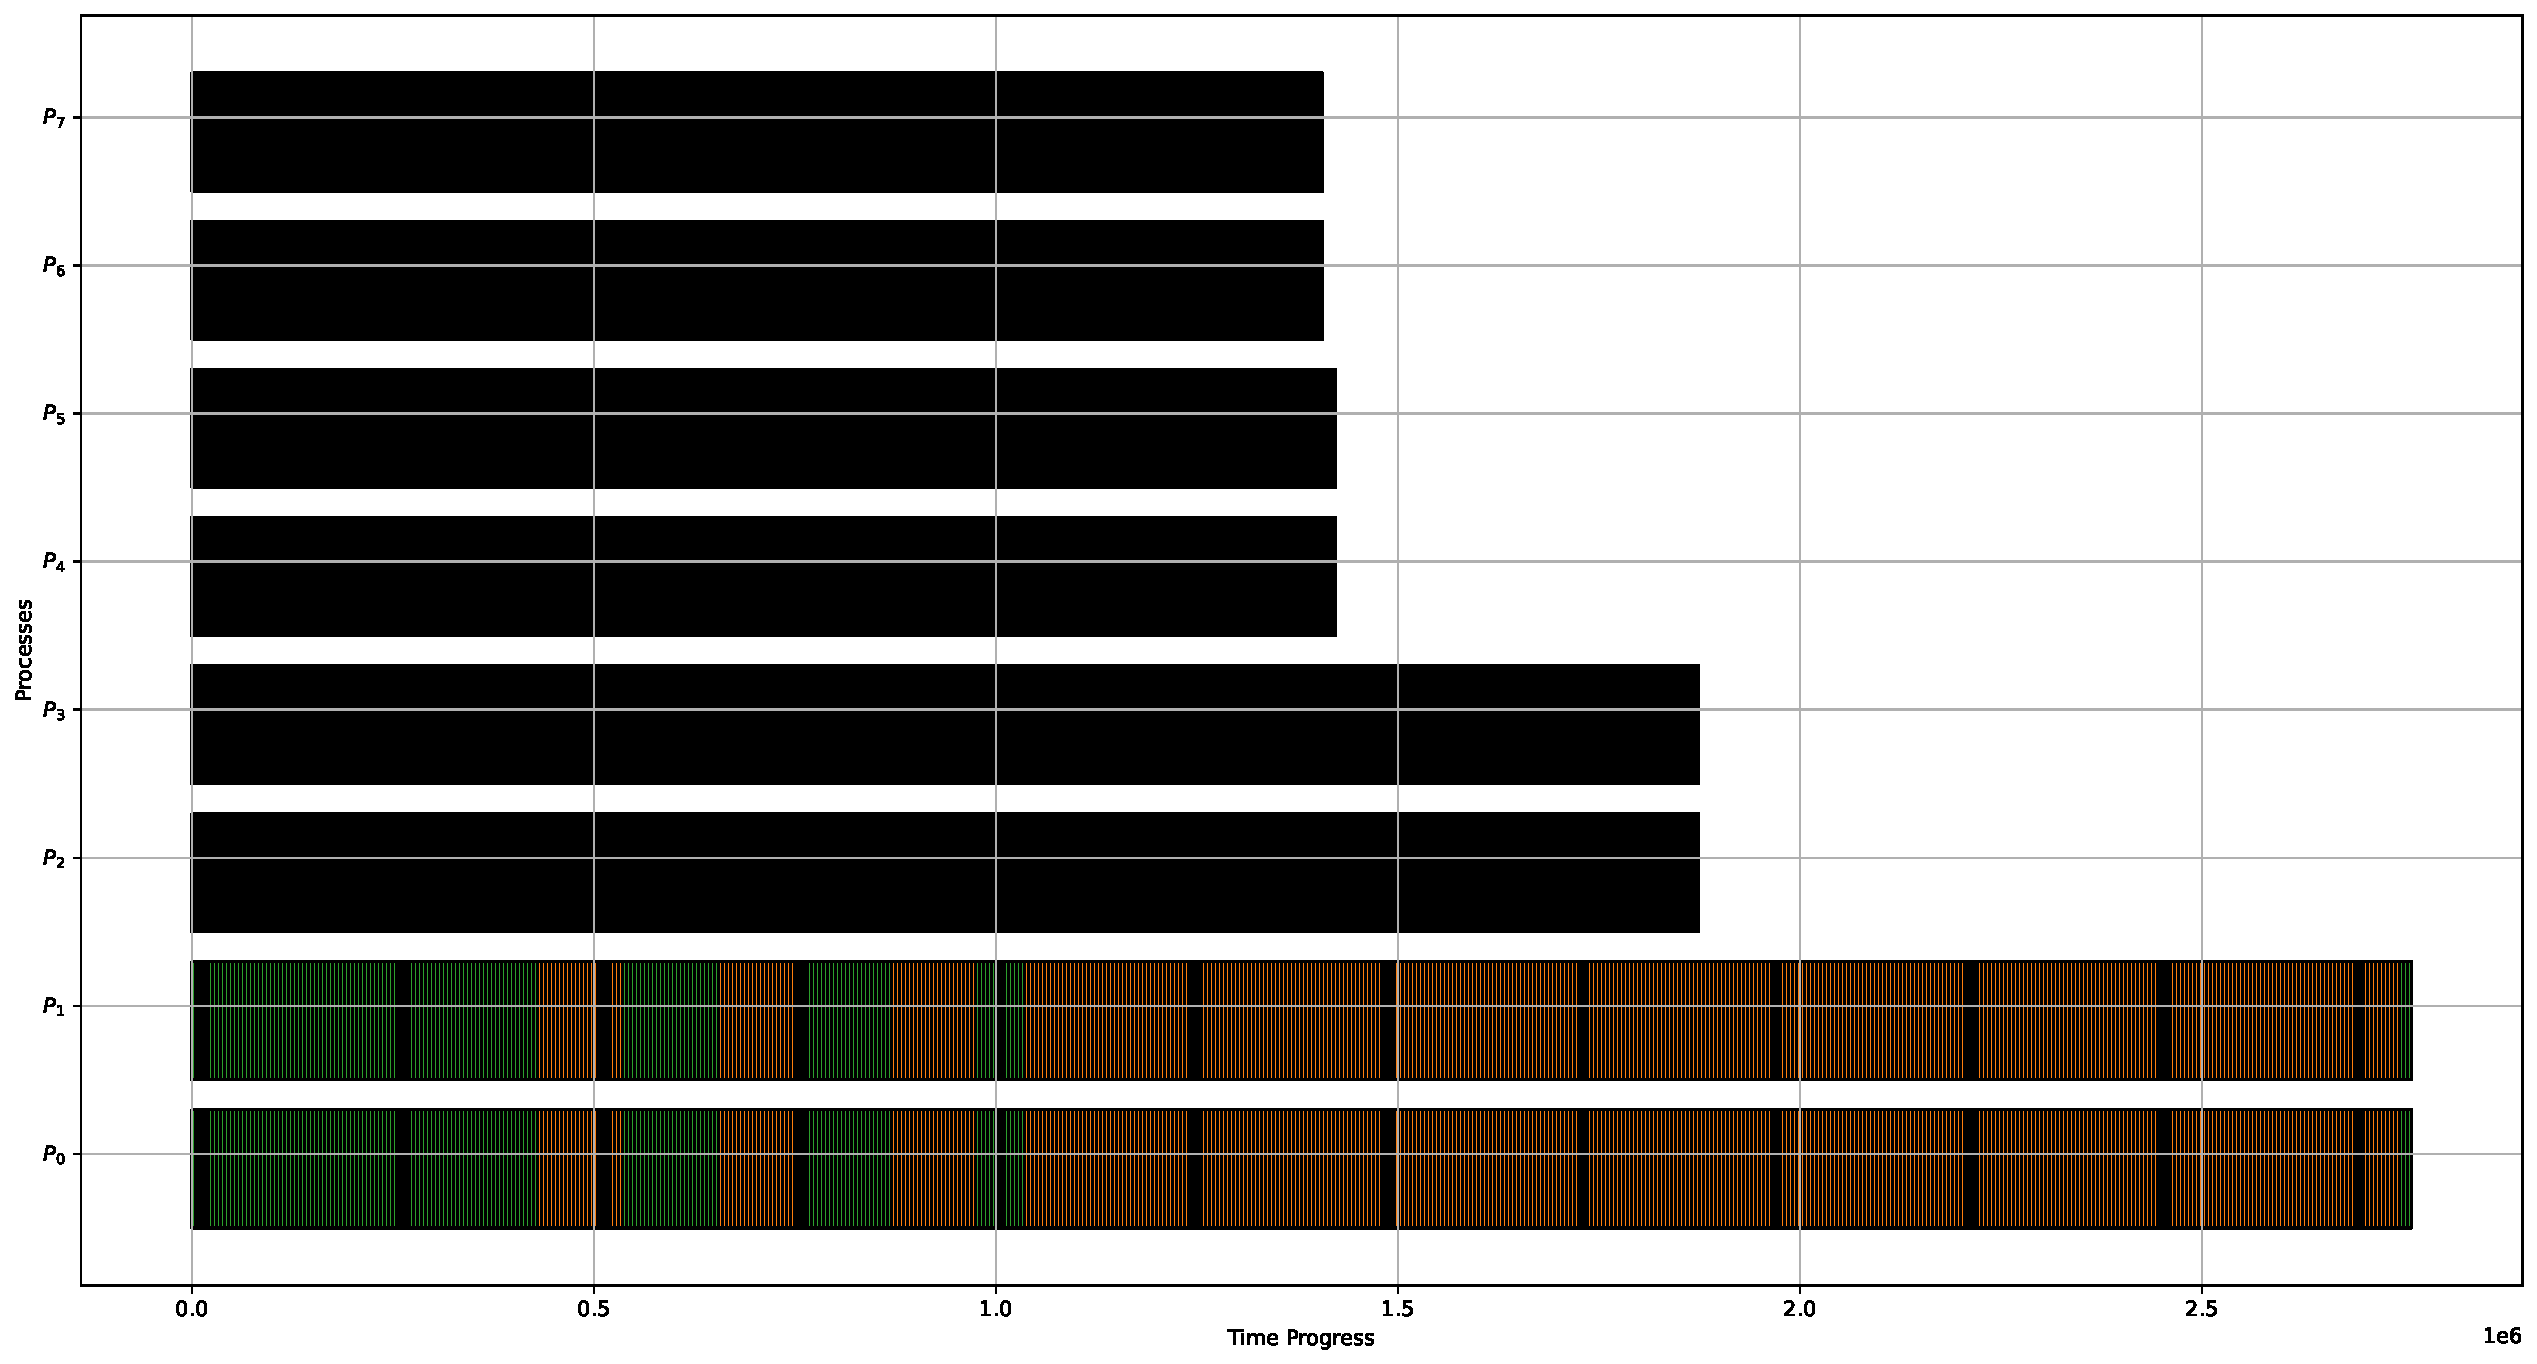
\includegraphics[scale=0.36]{./pictures/perf_analysis_model/perf_model_simulate_react_lb_1000_tasks_per_rank.pdf}
	\caption{An example simulation run with reactive load balancing in the scenario of $8$ processes, $1000$ tasks/process.}
	\label{fig:react_lb_simulation_1000_tasks_per_rank_example}
\end{figure}

Following the time steps and actions simulated for Scenario $1$, the module \texttt{Profiler} of our simulator can record the information, such as when tasks are queued and started execution, migration, termination, to profile the behavior of reactive load balancing. Typically, Figure \ref{fig:react_lb_simulation_1000_tasks_per_rank_example} depicts the profiled task execution over time progress by the simulator. The x-axis indicates time progress, while the y-axis indicates $8$ processes in this simulation scenario. We configure $8000$ tasks in total and $1000$ tasks/process as a given distribution. Process $P_{0}$ and process $P_{1}$ are the slowdown processes. With the given scale of $5 \times$ slower than normal, one task is executed in $5$ seconds. Without load balancing, the total load of process $P_{0}$ and $P_{1}$ would be $5000$s. Through applying reactive load balancing, we can see that the completion time is reduced to around $2700$s.\\

In Figure \ref{fig:react_lb_simulation_1000_tasks_per_rank_example}, a range of ``green'' slots indicates local task execution, while ``orange'' indicates remote task execution. Such an example simulator run, we simply configure the overhead information, consisting of:
\begin{itemize}
	\item Balancing operation overhead (named $O_{\text{balancing}}$): $20$ms occupied $2\%$ of task execution time unit. This means a task is executed in $1$s ($1000$ms), then balancing operations at once take $20$ms. As mentioned in Subsection \ref{subsec:discrete_time_model}, $O_{\text{balancing}}$ accounts for the time of monitoring ($m_{i}(t, t+\Delta t)$) and exchaning load information ($b_{i}(t - \lambda)$).
	\item Task migration overhead (represented by delay time $d$): $10$ms occupied $1\%$ of the task execution time unit.
\end{itemize}

As we can see in Figure \ref{fig:react_lb_simulation_1000_tasks_per_rank_example}, reactive task migration is sometimes incorrect because process $P_{0}$ and $P_{1}$ are known as overloaded processes but they still receive remote tasks. This also happens in a real execution with certain cases of high imbalance alongside many tasks per process and small execution time per task In Figure \ref{fig:react_lb_simulation_1000_tasks_per_rank_example} with the processes $P_{2}$, $...$, $P_{7}$, the area of local tasks is tight and overlaps together; therefore, we might not see clear local task execution. With process $P_{0}$ and $P_{1}$, the area of remote tasks is marked such incorrect task offloading at several time slots.\\

The following subsection provides further details about the evaluation of our simulator. We intend to show the impact between balancing operation overhead and task migration overhead. Notably, we address why reactive load balancing is late at runtime in distributed memory systems.

% We have these constraints to declaring imbalance context based on the number of involved processes ($P$), tasks ($T$), the scale of slowdowns such as $20\%$, $30\%$, or $50\%$, ..., then the number of processes being slow. The last input is the execution rate which denotes how many tasks can be done per time unit, or we can say how the throughput of execution (tasks/time unit) is.\\

% Below the \texttt{Simulation Engine spec.} region is an iteraction region, including \texttt{Balancer} and \texttt{Migrator}. Each time clocking, the balancer will check the queue's status for imbalance ratio ($R_{imb}$). If $R_{imb}$ meets the requirement of offloading tasks, it will signal \texttt{Migrator} for further actions to offloading tasks. Additionally, there is the second interaction region named \texttt{Profiler}. Before a time clock is closed, we can trigger the profiler to trace and record data for visualizing the simulation of our execution with dynamic load balancing. As we can see, the diagram extends the design in Figure \ref{fig:react_lb_simulator} to a communication diagram in more detail. Following the action arrows, we can determine the working flow from the points of simulation view. For example, after getting the imbalance context, we start with \texttt{queue\_setup()}, and \texttt{Clocking} is managed to proceed. Then, the behavior contineou by checking the queues (\texttt{check\_queue()}), ... until the termination of a loop (at \texttt{4.} \texttt{increase} \texttt{\_clock()}).\\

\subsection{Simulator Evaluation}
\label{subsec:Simulator-Evaluation}

\subsubsection{Example without load balancing}
\label{subsubsec:eval-sim-example-no-lb}

The simulation scenario in this subsection is similar to the previous example of Figure \ref{fig:react_lb_simulation_1000_tasks_per_rank_example}. However, we reduce the total number of tasks to reduce simulation time, where each process holds $100$ tasks. The imbalance ratio is also configured $R_{imb} = 1.5$, $P = 8$ processes, and below is an input sample for configuring the simulator.

\begin{lstlisting}[language=Python, caption={Input sample for the baseline simulation.}, label={lst:sim_input_sample}]
	num_process: 8
	num_tasks:   800
	slowdown:    0.2 # the scale of slowdown
	num_sld_processes: 2 # the number of slowed processes
	bandwidth: 1485 MB/s # bandwidth value for calculating delay
	exe_rate: 1.0 task/s # the execution rate
\end{lstlisting}
\hfill

\begin{figure}[t]
  \centering
  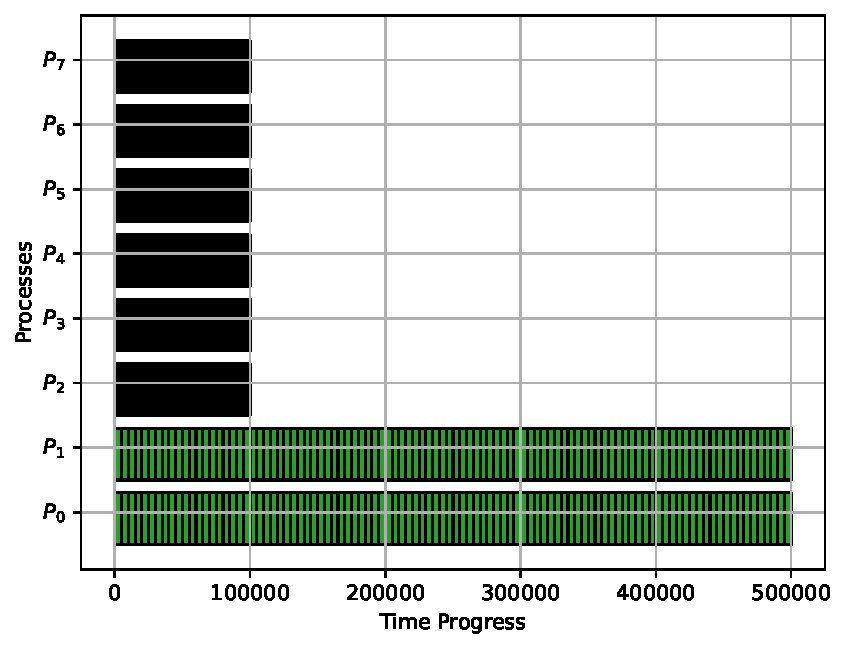
\includegraphics[scale=0.65]{./pictures/poc_implementation/poc_visualize_baseline_case_8_processes.pdf}
	\caption{Visualization of the baseline simulation without load balancing.}
	\label{fig:simulator_baseline_case}
\end{figure}

This input is used to simulate the baseline without load balancing. Technically, module \texttt{Balancer} is deactivated in this case. Therefore, there are no values for balancing operation overhead and task migration overhead. With time steps in milliseconds (ms), the clock is counted one by one at a time. In normal processes, the execution rate is $1.0$ task/s, and the total load value of each is ideally $100$s. In slowdown processes, the execution rate is $0.2$, where we simply set process $P_{0}$ and $P_{1}$ as the slow processes. Executing each task in process $P_{0}$ and $P_{1}$ takes $5$s. The completion time without load balancing is $500$s in total. Figure \ref{fig:simulator_baseline_case} shows the simulated baseline. The x- and y-axis also point to the time progress and the load-value bars of $8$ processes. Green boxes denote the executed tasks that are clearly seen at process $P_{0}$ and process $P_{1}$. The load values on other processes are smaller compared to process $P_{0}$ and $P_{1}$ due to many overlapped tasks. Hence, we might see task execution on their sides black (not clearly green as expected).\\

The following is a detailed statistic output from our simulator (Listing \ref{lst:sim_output_sample}). First, the configuration information (under the block \texttt{Configuration}) is summarized. Second, under the block \texttt{Executed Tasks}, the output summarizes the number of local and remote tasks executed on each process. Then, the blocks \texttt{Total Load} and \texttt{Statistic} summarize the total load values of processes and the corresponding maximum, minimum, average load values, resulting in the imbalance ratio. Overall, the detailed output and profiled data can be directed to a \texttt{csv}-format file.

\begin{lstlisting}[language=Python, caption={The output of the baseline simulation.}, label={lst:sim_output_sample}]
-------------------------------------------
Configuration
-------------------------------------------
   + num. processes:     8
   + num. tasks:       800
   + slowdown:         0.2
   + num. sld.procs:     2
   + bandwidth:      1485.0 (MB/s)
   + exe_rate:         1.0 (task/s)
-------------------------------------------

-------------------------------------------
Summary: Executed Tasks
-------------------------------------------
	 + P[0]: num.local_tasks=  100, num.remote_tasks=    0
	 + P[1]: num.local_tasks=  100, num.remote_tasks=    0
	 + P[2]: num.local_tasks=  100, num.remote_tasks=    0
	 + P[3]: num.local_tasks=  100, num.remote_tasks=    0
	 + P[4]: num.local_tasks=  100, num.remote_tasks=    0
	 + P[5]: num.local_tasks=  100, num.remote_tasks=    0
	 + P[6]: num.local_tasks=  100, num.remote_tasks=    0
	 + P[7]: num.local_tasks=  100, num.remote_tasks=    0
-------------------------------------------

-------------------------------------------
Summary: Total Load
-------------------------------------------
   + P[0]: local_load= 500.00(s), remot_load=   0.00(s)
   + P[1]: local_load= 500.00(s), remot_load=   0.00(s)
   + P[2]: local_load= 100.00(s), remot_load=   0.00(s)
   + P[3]: local_load= 100.00(s), remot_load=   0.00(s)
   + P[4]: local_load= 100.00(s), remot_load=   0.00(s)
   + P[5]: local_load= 100.00(s), remot_load=   0.00(s)
   + P[6]: local_load= 100.00(s), remot_load=   0.00(s)
   + P[7]: local_load= 100.00(s), remot_load=   0.00(s)
-------------------------------------------

-------------------------------------------
Statistic
-------------------------------------------
max. load:   500.0
min. load:   100.0
avg. load:   200.0
R_imb:         1.5
sum. overloaded_load:    600.0
sum. underloaded_load:   600.0
-------------------------------------------
Write profiled queue data to: ./poc_visualize_baseline_case_8_procs_output.csv
-------------------------------------------
\end{lstlisting}
\hfill

\subsubsection{Example with reactive load balancing}
\label{subsubsec:eval-sim-example-reactlb}

In the case of applying reactive load balancing, we activate \texttt{Balancer} and configure the values for balancing operation overhead and task migration overhead. With a simulation trial, we initially set the balancing overhead, $O_{\text{balancing}} = 1.0$ms, and delay time, $d=1.0$ms. Compared to the execution time unit of a task in second, we highlight that balancing overhead and delay time occupy $0.1\%$.\\

\begin{figure}[t]
  \centering
  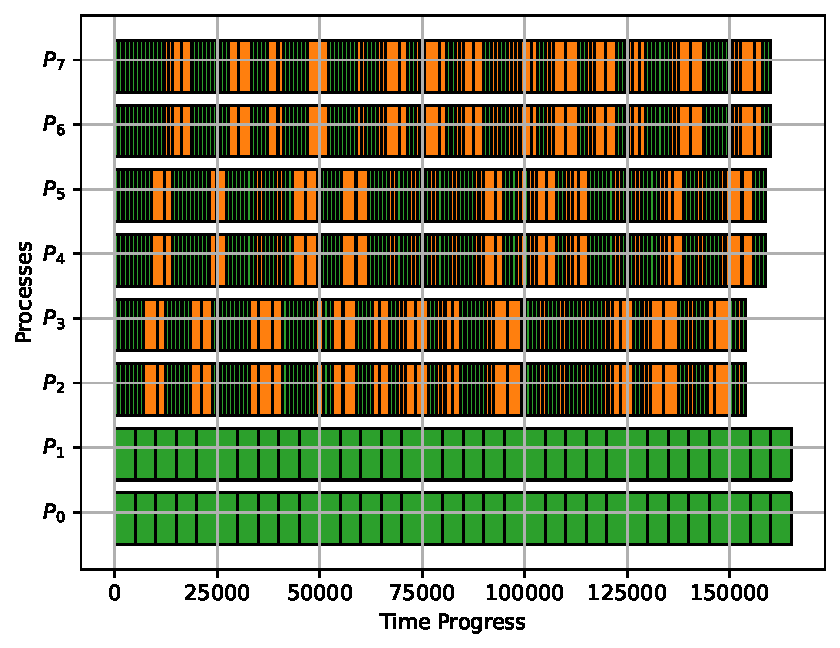
\includegraphics[scale=0.65]{./pictures/poc_implementation/poc_visualize_reactlb_O1_d1_8_processes.pdf}
	\caption{Visualiztion of reactive load balancing case of simulation with $O_{\text{balancing}} = 1.0$ms and $d=1$ms.}
	\label{fig:simulator_reactlb_O1_d1_case}
\end{figure}

Figure \ref{fig:simulator_reactlb_O1_d1_case} shows the visualization of the simulation with reactive load balancing, where $O_{\text{balancing}} = 1.0$ms and $d = 1.0$ms. The x- and y-axis shows time progress and processes executing tasks, where ``green'' and ``orange'' slots indicate local can remote tasks. Overall, the completion time is reduced. The simulated operations of reactive task offloading with $O_{\text{balancing}}$ and $d$ are acted as follows.
\begin{itemize}
	\item Suppose at a time $t_{k}$, module \texttt{Balancer} detects an imbalance and tasks from process $P_{0}$ are then offloaded to process $P_{7}$ as an example. However, the tasks are proceeded in the queue for offloading at time $t_{k} + 1$ because of $O_{\text{balancing}} = 1.0$.
	\item Similarly, assuming tasks from process $P_{0}$ are decided to offload to process $P_{7}$ at $t_{k}$. However, these tasks arrive at process $P_{7}$ at time $t_{k} + 1$ because of $d = 1.0$.
\end{itemize}

In the simulator, module \texttt{Clocking} controls the ticking procedure of time steps. We can adjust this procedure to simulate the execution of dynamic load balancing similar to running in practice. Listing \ref{lst:sim_output_reactlb_O1_d1} shows the output sample of this simulated scenario. The output format is equivalent to Listing \ref{lst:sim_output_sample}, but we skip the part of \texttt{Configuration}. As a result, the summary under block \texttt{Executed Tasks} highlights the number of remote tasks from process $P_{2}$ to $P_{7}$. In response to the number of remote tasks, block \texttt{Total Load} indicates the total load values of remote tasks, proving that reactive load balancing works. In the end, the completion time is improved significantly $\approx 165.0$ms, and $R_{imb}$ is almost $0.0$.

\begin{lstlisting}[language=Python, caption={The simulation output of reactive load balancing with $O_{\text{balancing}} = 1.0$ms, $d=1$ms}, label={lst:sim_output_reactlb_O1_d1}]
-------------------------------------------
Configuration
-------------------------------------------
   ...
-------------------------------------------

-------------------------------------------
Summary: Executed Tasks
-------------------------------------------
	 + P[0]: num.local_tasks=   33, num.remote_tasks=    0
	 + P[1]: num.local_tasks=   33, num.remote_tasks=    0
	 + P[2]: num.local_tasks=   82, num.remote_tasks=   38
	 + P[3]: num.local_tasks=   82, num.remote_tasks=   38
	 + P[4]: num.local_tasks=   81, num.remote_tasks=   42
	 + P[5]: num.local_tasks=   81, num.remote_tasks=   42
	 + P[6]: num.local_tasks=   76, num.remote_tasks=   48
	 + P[7]: num.local_tasks=   76, num.remote_tasks=   48
-------------------------------------------
	
-------------------------------------------
Summary: Total Load
-------------------------------------------
   + P[0]: local_load= 165.00(s), remot_load=   0.00(s)
   + P[1]: local_load= 165.00(s), remot_load=   0.00(s)
   + P[2]: local_load=  82.00(s), remot_load=  72.50(s)
   + P[3]: local_load=  82.00(s), remot_load=  72.50(s)
   + P[4]: local_load=  81.00(s), remot_load=  75.00(s)
   + P[5]: local_load=  81.00(s), remot_load=  75.00(s)
   + P[6]: local_load=  76.00(s), remot_load=  81.00(s)
   + P[7]: local_load=  76.00(s), remot_load=  81.00(s)
-------------------------------------------

-------------------------------------------
Statistic:
-------------------------------------------
max. load:   165.0
min. load:   154.5
avg. load:   158.1
R_imb:         0.0
sum. overloaded_load:     13.8
sum. underloaded_load:    13.8
-------------------------------------------
Write profiled queue data to: ./profiled_queues_reactlb_O1_d1.csv
-------------------------------------------
\end{lstlisting}

\subsubsection{Experiments with the simulator}
\label{subsubsec:eval-sim-experiments-reactlb}

\begin{figure}[t]
\centering
\subfloat[Subfigure1][Reactive LB with $O_{\text{balancing}}$ $=2$ms and $d=2$ms]{
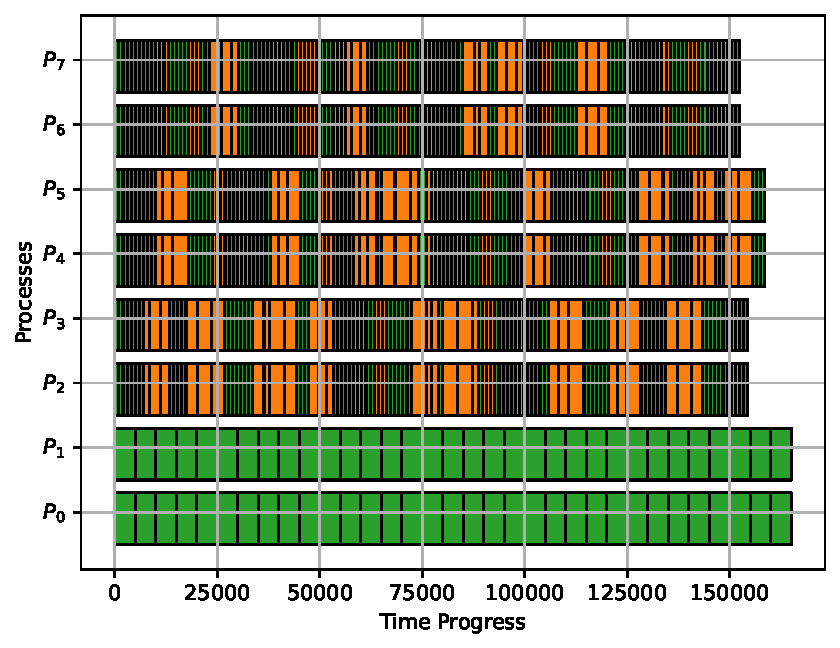
\includegraphics[scale=0.525]{./pictures/poc_implementation/poc_visualize_reactlb_O2_d2_8_processes.pdf}
\label{sfig:reactlb_O2_d2}}
\subfloat[Subfigure2][Reactive LB with $O_{\text{balancing}}$ $=5$ms and $d=2$ms]{
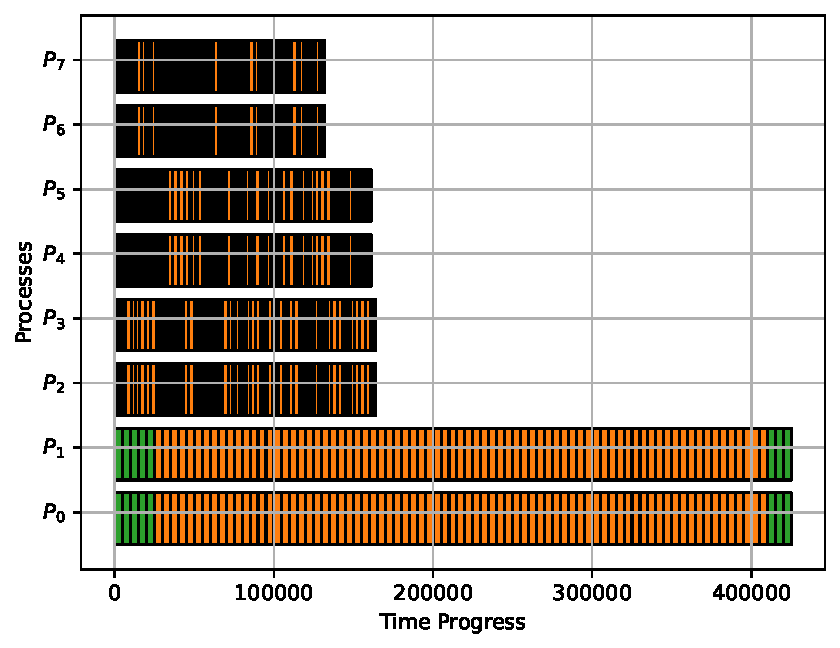
\includegraphics[scale=0.525]{./pictures/poc_implementation/poc_visualize_reactlb_O5_d2_8_processes.pdf}
\label{sfig:reactlb_O5_d2}}
\qquad
\subfloat[Subfigure3][Reactive LB with $O_{\text{balancing}}$ $=10$ms and $d=2$ms]{
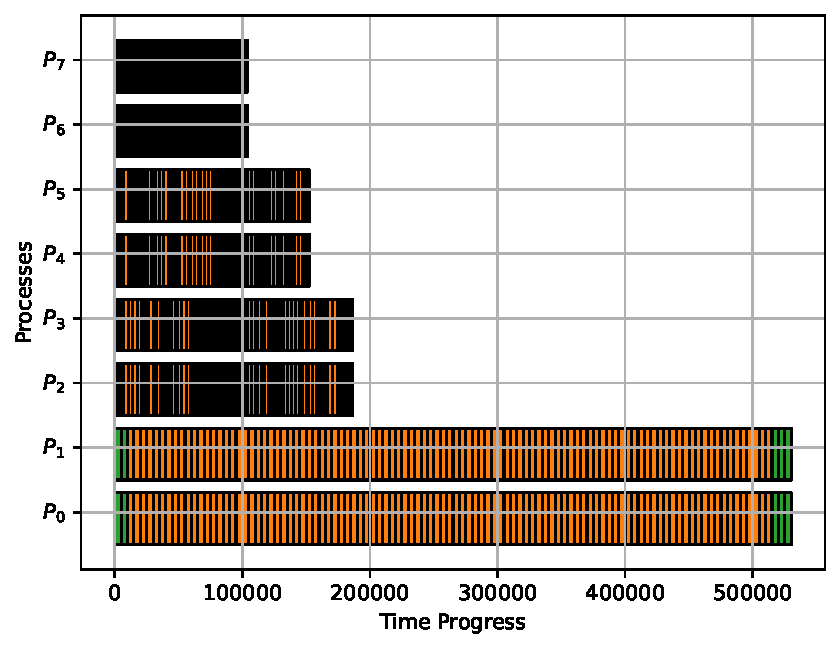
\includegraphics[scale=0.525]{./pictures/poc_implementation/poc_visualize_reactlb_O10_d2_8_processes.pdf}
\label{sfig:reactlb_O10_d2}}
\subfloat[Subfigure4][Reactive LB with $O_{\text{balancing}}$ $=20$ms and $d=2$ms]{
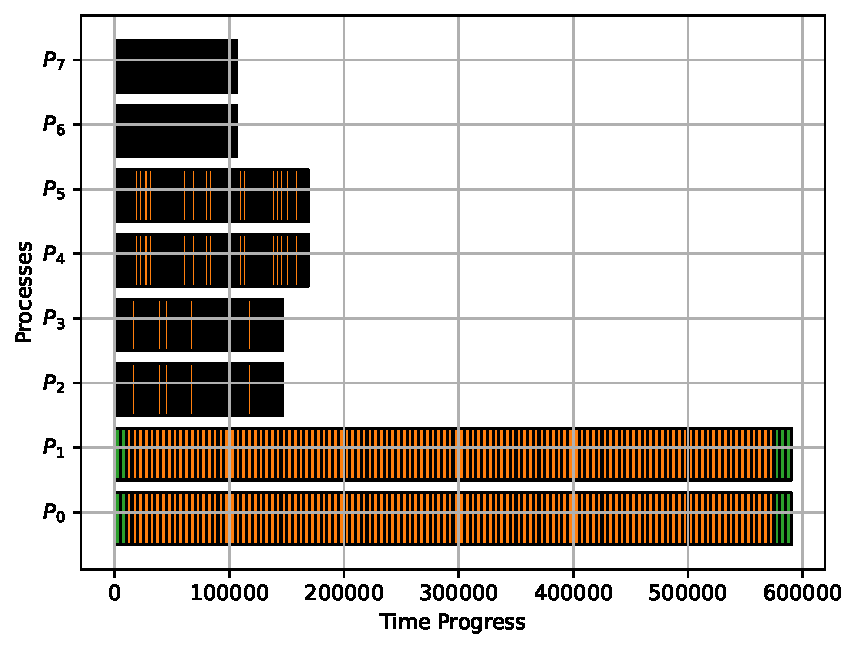
\includegraphics[scale=0.525]{./pictures/poc_implementation/poc_visualize_reactlb_O20_d2_8_processes.pdf}
\label{sfig:reactlb_O20_d2}}
\caption{A visualization of reactive load balancing with increased balancing overhead and delay.}
\label{fig:simulator_reactlb_increased_Ovaried_d2}
\end{figure}

To see the effects of balancing overhead, we try to increase $O_{\text{balancing}}$ first from $2$, $5$, $10$, to $20$ms, corresponding to the occupation of $0.2\%$, $0.5\%$, $1.0\%$, $2.0\%$ over task execution time unit, while $d = 2$ is kept constantly. Figure \ref{fig:simulator_reactlb_increased_Ovaried_d2} shows these tests in the visualization of reactive load balancing (denoted by Reactive LB). Compared to the baseline (in Figure \ref{fig:simulator_baseline_case} on Page \pageref{fig:simulator_baseline_case}) and the initial imbalance scenario (in Figure \ref{fig:simulator_reactlb_O1_d1_case} on Page \pageref{fig:simulator_reactlb_O1_d1_case} with $O_{\text{balancing}}$ $=1$ms, $d=1$ms), Figure \ref{fig:simulator_reactlb_increased_Ovaried_d2} highlights the impact of balancing operation overhead. Not only delay time, load balancing operations in monitoring, exchanging load information/queue status, and calculating imbalance conditions can also significantly affect overall performance. $O_{\text{balancing}}$ is sensitive when almost all dynamic load balancing methods decide on many continuous actions and task migrations. For instance, the balancing decisions start getting worse when $O_{\text{balancing}}$ occupies $0.5\%$ over task execution time unit.\\

\begin{figure}[t]
\centering
\subfloat[Subfigure1][Reactive LB in that keep $O_{\text{balancing}}=2$ constantly and vary $d$]{
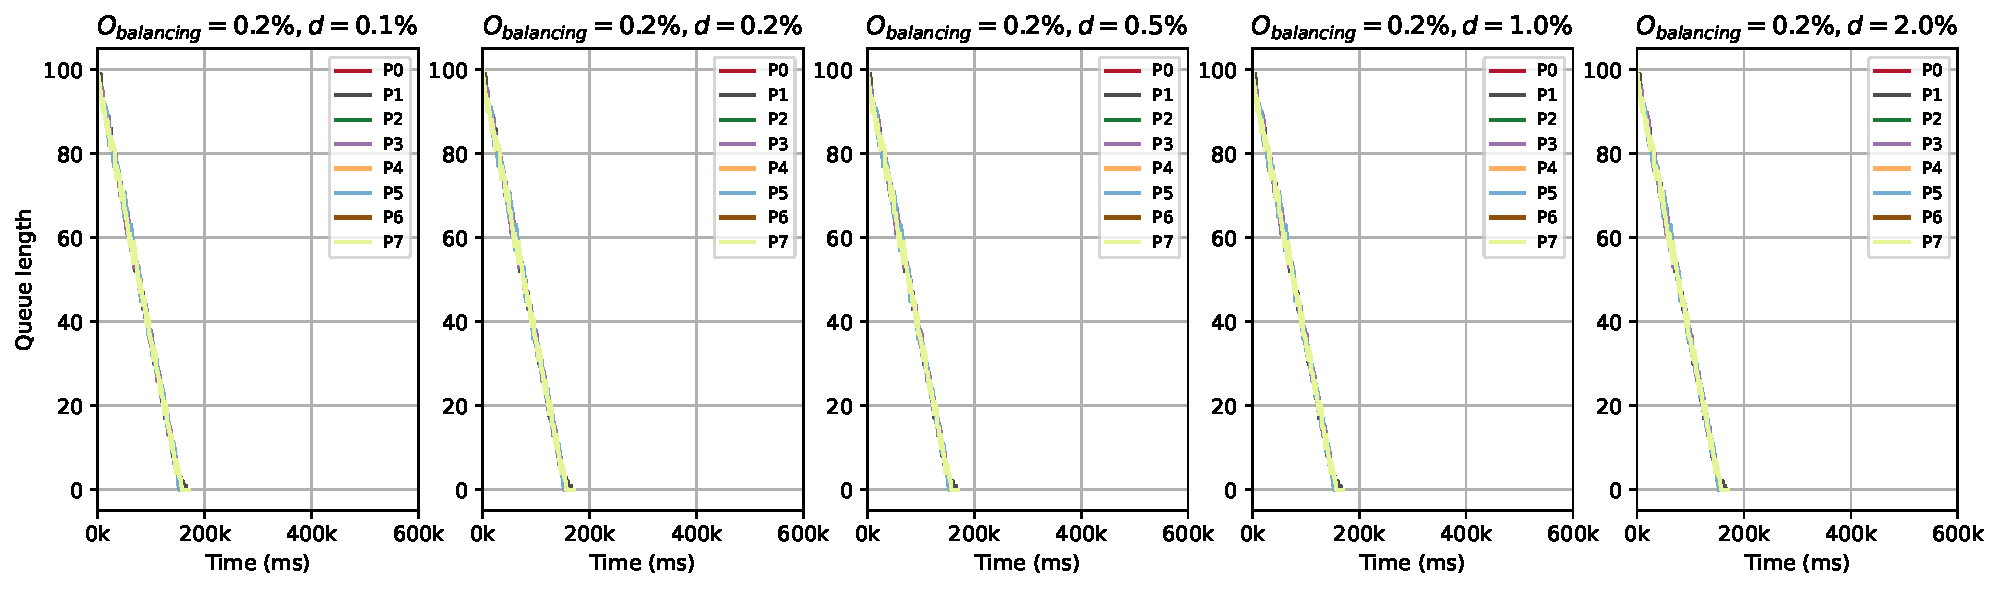
\includegraphics[scale=0.4]{./pictures/perf_analysis_model/perf_model_queue_decrease_delay_impact_OB2.pdf}
\label{sfig:reactlb_O2_dvaried}} \\

\subfloat[Subfigure2][Reactive LB in that keep $O_{\text{balancing}}=5$ constantly and vary $d$]{
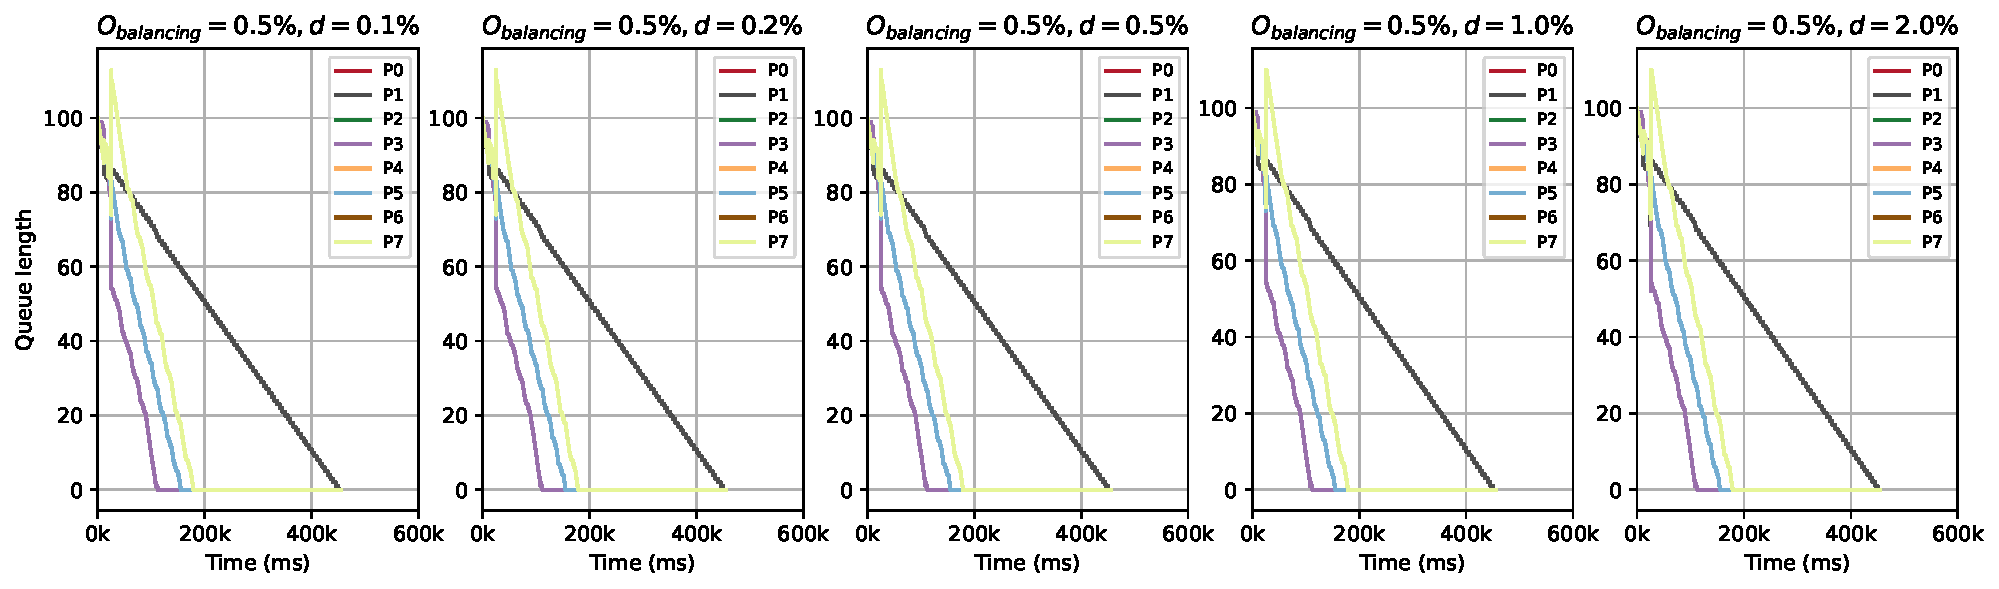
\includegraphics[scale=0.4]{./pictures/perf_analysis_model/perf_model_queue_decrease_delay_impact_OB5.pdf}
\label{sfig:reactlb_O5_dvaried}} \\

\subfloat[Subfigure3][Reactive LB in that vary $O_{\text{balancing}}$ and keep $d=2$ constantly]{
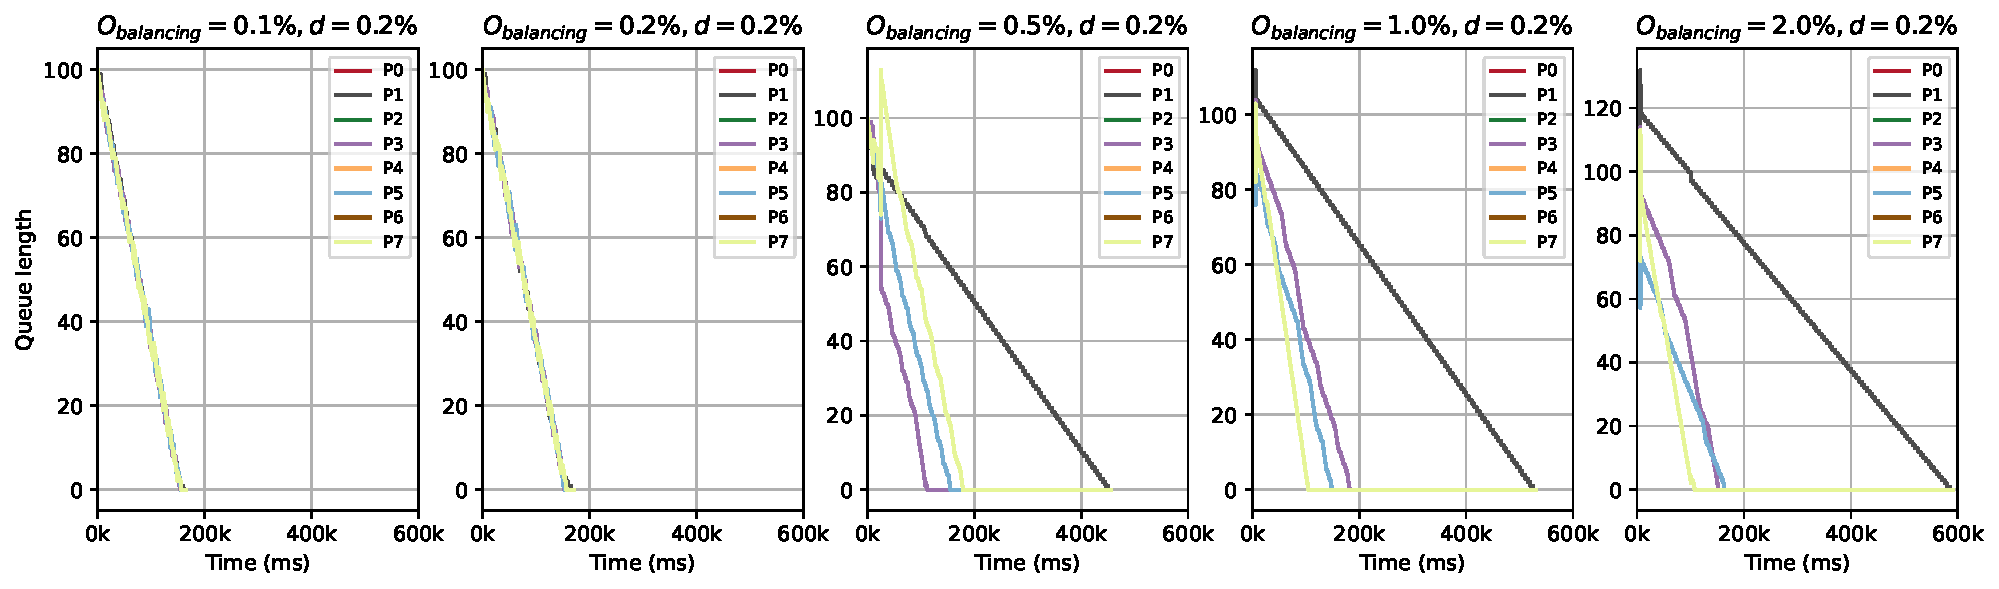
\includegraphics[scale=0.4]{./pictures/perf_analysis_model/perf_model_queue_decrease_blancing_impact_d2.pdf}
\label{sfig:reactlb_Ovaried_d2}}

\caption{Evaluation of the queue length convergence when varying task migration overhead (delay) and balancing operation overhead.}
\label{fig:evaluation_Obalancing_effects}
\end{figure}

For another evaluation, we keep $O_{\text{balancing}}$ as a constant and vary $d$ to see the impact of task migration overhead, Figure \ref{fig:evaluation_Obalancing_effects} shows two experiments conducted, one in Figure \ref{sfig:reactlb_O2_dvaried} showing $O_{\text{balancing}}=2$ and $d$ is ranged from $0.1\%$ to $2\%$; one in Figure \ref{sfig:reactlb_O5_dvaried} showing $O_{\text{balancing}}=5$ and $d$ is ranged from $0.1\%$ to $2\%$. The imbalance scenario is stayed similar to the previous tests. In both figures, the x-axis indicates the progress of queues changed over time steps (in ms); the y-axis indicates the queue length as the number of remaining tasks over time steps.\\

Generally, all the queues are converged into $0$ at the end after the execution is finished. However, the slope of different queue lines might be different because some processes are slowed down and execute tasks slower. Note that these experiments with the simulator are applied reactive load balancing, and the final results show the load balancing performance. Typically, the slope in these figures represents how efficient the performance is. The last queue converged at shorter time steps determines a better performance. The balancing operation overhead is still trivial with $O_{\text{balancing}}=2$. We can see that increasing $d$ does not affect the convergence speed much. However, with $O_{\text{balancing}}=5$, delay $d$ here is more sensitive, and the convergence of queues gets impacted. Following this, if we compare with the experiments visualized in Figure \ref{fig:simulator_reactlb_increased_Ovaried_d2} (on Page \pageref{fig:simulator_reactlb_increased_Ovaried_d2}) when $d$ is constant and $O_{\text{balancing}}$ is varied, Figure \ref{sfig:reactlb_Ovaried_d2} emphasizes in detail these scenarios with the convergence of queue lengths. For a slightly change of $O_{\text{balancing}}$, the load balancing performance is significantly affected.

